

\input{../Latex_Templates/Preamble_Report}

%%%%% TITLE PAGE

%\subject{, VT23}
\title{Some relations between equilibria of harmonic vector fields and the domain topology. \\[1ex]
	  \large Master Thesis}
%\subtitle{}
\author{Theo Koppenhöfer}
\date{Lund \\[1ex] \today}

\addbibresource{bibliography.bib}

\usepackage{svg}
\graphicspath{{../Plots/}}
\graphicspath{{../Figures/}}

\usepackage{makecell}
\newcounter{symbolCount}
\newcommand{\nomenclature}[2]{\stepcounter{symbolCount}
\glsxtrnewsymbol[description={#2}]{\arabic{symbolCount}}{#1}}
\usepackage[symbols,
  stylemods={tree},% loads glossaries-extra-stylemods to patch styles
  record, % using 'bib2gls'
  nonumberlist
]{glossaries-extra}

% % assign titles to group labels: 
% \glsxtrsetgrouptitle{latin}{Latin}
% \glsxtrsetgrouptitle{greek}{Greek}

% \GlsXtrLoadResources[
%  src={symbolsList.bib},
%  type=symbols,
% %  group={latin},% assign group label
% %  set-widest,% needed for 'alttree' styles
%  save-locations=false
% ]

% \glsxtrnewsymbol[description={velocity}]{v}{\ensuremath{v}}



% The following displays the labels, uncomment for final version
% \usepackage{showlabels}

\newcommand{\bx}{\bar{x}}
\renewcommand{\chaptername}{Section}

%%%%% The content starts here %%%%%%%%%%%%%


\begin{document}

\maketitle

\tableofcontents

\newpage

\listoftodos

\todoin[]{
  General TODOs
  \begin{itemize}
    \item Check for typos.
    \item Does Girault-Raviart theorem with Helmholtz decomp. help?
    \item bring in results from \cite{Shelton1980} and \cite{Morse1970}
    \item Harmonic vector fields, find up to date reference
    \item Mention Sard's theorem
    \item Does Bocher's theorem help?
    \item Generalise argument principle proof to one inflow, outflow
    \item Look at application of Sperner's lemma
    \item $C$ is used once for critical points, once for level sets.
  \end{itemize}
  Some questions
  \begin{itemize}
    \item Should I state Hopf's Lemma?
    \item Weak formulation - a distraction? \textrightarrow Hartman, Wintner
  \end{itemize}
}

\newpage

\section{Introduction}

\ruggedtodo[inline]{Some amazing introduction}

Unless otherwise stated we denote by $\Omega\subseteq\R^d$ an open bounded subset of $\R^d$ with boundary $\Sigma=\partial\Omega$.
\nomenclature{$d$}{Dimensions $d=2$ or $d=3$}
\nomenclature{$\Omega$}{Domain in $\R^d$}
\nomenclature{$\Sigma$}{Boundary of $\Omega$, often assumed to be a $C^2$ manifold}
In the following we will work in dimensions $d\in\brk[c]{2,3}$.
We denote with
\begin{align*}
  f\colon\overline{\Omega}\to\R
\end{align*}
a scalar function of class $C^2$.
\nomenclature{$f\colon \overline{\Omega}\to\R$}{A $C^2$ mapping, often assumed harmonic}
We also denote by
\begin{align*}
  u\colon\overline{\Omega}\to\R^d
\end{align*}
a vector field of class $C^1$.
\nomenclature{$u\colon \overline{\Omega}\to\R^d\text{ or }T^*\overline{\Omega}$}{A $C^1$ vector field, often assumed harmonic}
Often but not always $u$ can be thought of as 
a \emph{harmonic vector field}, that is $u$ is of type $C^1$ and fulfils
\begin{align*}
  \diver u=0 \qquad \text{ and }\qquad \curl u=0\,.
\end{align*}
Also often but not always we assume that globally $u=\nabla f$ is a gradient field, implying that $f$ is harmonic.
One question we seek to answer during this thesis is the following.
\begin{question}[Flowthrough with stagnation point]\label{qu:flowthroughStagnationPoint}
  Does there exist a tube $\Omega\subseteq\R^3$ with flow $u$ through the tube such that
  \begin{enumerate}
    \item $u$ is a harmonic vector field
    \item $u$ has an interiour stagnation point
    \item $u$ enters the tube on the one side and exits the tube on the other?
  \end{enumerate}
\end{question}
To make the formulation more precise we begin with some general definitions regarding stagnation points and the boundary conditions.

\subsection{General definitions}

In the following we define the emergent and the entrant boundary as in \cite[p.282]{Morse1970}
\begin{definition}[Emergent and entrant boundary]\label{df:emergentEntrantBd}
  We call a vector $v\in T_x\R^d$ \emph{entrant} at a boundary point $x\in\Sigma$ iff $v$ is not tangent to $\Sigma$
  and directed into the interiour of $\Omega$. Analogously if $v$ is not tangent and
  directed to the exteriour we call $v$ \emph{emergent}.
  We define the \emph{entrant boundary} $\Sigma^-$ to be the set of boundary points at which $u$ is entrant.
  Analogously define the \emph{emergent boundary} $\Sigma^+$ to be the set of boundary points at which
  $u$ is emergent.
  Further define the \emph{tangential boundary} $\Sigma^0$ to contain all other boundary points such that we have a decomposition
  of the boundary
  \begin{align*}
    \Sigma=\Sigma^-\sqcup\Sigma^0\sqcup\Sigma^+\,.
  \end{align*}
\end{definition}
\nomenclature{$\Sigma^-$}{entrant boundary, see definition \ref{df:emergentEntrantBd}}
\nomenclature{$\Sigma^+$}{emergent boundary, see definition \ref{df:emergentEntrantBd}}
\nomenclature{$\Sigma^0$}{tangential boundary, see definition \ref{df:emergentEntrantBd}}
\tdrewrite{Use differential topology language in the following section.}

We would now like to illustrate the preceeding definitions.
\begin{example}\label{ex:n3_hvf_canonical}
  We now consider our domain to be the ball $B_1\subseteq\R^3$ around the origin in $d=3$ dimensions.
  Now consider the harmonic function
  \begin{equation}
    \begin{aligned}
    f\colon \Omega&\to\R \\
    x&\mapsto x_1^2+x_2^2-2x_3^2\label{eq:n3_hf_canonical}
    \end{aligned}
  \end{equation}
  Which induces the harmonic vector field $u=\nabla f$, or more precisely
  \begin{equation}
    \begin{aligned}
    u\colon \Omega&\to\R \\
    x&\mapsto \vect{2x_1 & 2x_2 & -4x_3}^\top\,.\label{eq:n3_hvf_canonical}
    \end{aligned}
  \end{equation}
  We have that the normal to the boundary $\Sigma=S^2$ is given by
  \begin{align*}
    n\colon S^2&\to S^2 \\
    x&\mapsto x
  \end{align*}
  and thus we have that $x\in\Sigma^-$ iff 
  \begin{align*}
    0>n\cdot u = 2\brk*{x_1^2+x_2^2-2x_3^2}=2f(x)
  \end{align*}
  A plot of the sets can be seen in figure \ref{pl:n3_hvf_canonical_boundary}.
  \begin{figure}
    \centering
    \missingfigure[figwidth=0.7\textwidth]{}
    \caption{Plots of the entrant, emergant and tangential boundary for the
      function $f$ given by equation \eqref{eq:n3_hf_canonical}}
    \label{pl:n3_hvf_canonical_boundary}
  \end{figure}
\end{example}

The following are slight generalisation of definitions given in \cite[p.138f]{Shelton1980}, \cite[§5]{Morse1969} and \cite[p.282f]{Morse1970}
to include harmonic vector fields.
\begin{definition}[Non-degeneracy]\label{df:nonDegeneracy}
  Let $v\colon X\to T^*X$ be a $C^1$ vector field on an $s$ dimensional $C^2$ manifold (with possibly boundary) $X$.
  Here $T^*X$ denotes the
  cotangent bundle of $X$ as defined for example in \cite[Chapter 6]{Hirsch1994}.
  We can think of $X\in\brk[c]*{\Omega,\Sigma}$.
  We call the zeroes of $v$ \emph{stagnation points}. A stagnation point $x\in X$ is called
  \emph{non-degenerate} if the derivative $$Dv(x)=Dv_x\in T_xT^*X\cong \R^{s\times s}$$ is bijective. We say that $x$ has \emph{index} $k$
  if $Dv(x)$ has exactly $k$ negative eigenvalues. $v$ is called \emph{non-degenerate} if all its stagnation points
  are non-degenerate.
\end{definition}
\nomenclature{$X,Y$}{arbitrary $C^s$ manifolds, potentially with boundary}

We first set $u=v$ and $X=\overline{\Omega}$ in the preceeding definition to obtain
\begin{definition}[Interiour type numbers]
  We call the stagnation points of $u$ \emph{interiour stagnation points}.
  The \emph{interiour type numbers} $M_k$ are defined to be
  the number of stagnation points of $u$ of index $k$.
  \nomenclature{$M_k$}{Interiour type numbers}
  The total number of interiour stagnation points is thus given by
  \begin{align*}
    M=\sum_kM_k\,.
  \end{align*}
  \nomenclature{$M$}{Total number of stagnation points}
\end{definition}

We call $\Omega$ a \emph{regular domain} if $\Sigma$ is a manifold of class $C^2$.
In the following definition we require $\Omega$ to be regular.
For a boundary point $x$ let $$\pi_x\colon \R^d\cong T_x\R^d\to T_x\Sigma$$ denote the orthogonal projection of a
vector at $x$ onto the tangent space of $\Sigma$ at $x$.
Let 
\begin{align}
  \tiu=\pi\circ u\vert_{\Sigma}\in C^1\brk*{T\Sigma}\label{eq:definitions:projectionSigma}
\end{align}
be the restriction and orthogonal projection of $u$ onto the tangent bundle of $\Sigma$.
We now apply definition \ref{df:nonDegeneracy} to $X=\Sigma$ and $v=\tiu$.
\begin{definition}[Boundary type numbers]\label{df:bdTypeNbrs}
  We define the \emph{boundary type numbers} $\mu_k$ to be
  the number of stagnation points of $u_{\Sigma^-}$ on the entrant boundary
  $\Sigma^-$ of index $k$.
  We further write $\nu_k$ for the $k$-th boundary type number of $-u$.
\end{definition}
\nomenclature{$\mu_k$}{boundary type numbers of $f$, see definition \ref{df:bdTypeNbrs}}
\nomenclature{$\nu_k$}{boundary type numbers of $-f$, see definition \ref{df:bdTypeNbrs}}
\nomenclature{$\tiu$}{restriction and orthogonal projection of $u$ onto $\Sigma$, see definition \ref{df:bdTypeNbrs}}

We now call $u$ \emph{regular} iff $u$, $\tiu$ and $-\tiu$ are non-degenerate and all stagnation points of $u$ lie in $\Omega$.

The previous definitions translate naturally to $f$.
That is we call $f$ regular, non-degenerate, et cetera iff $u=\nabla f$ is regular, non-degenerate, et cetera.
Similarly we call $x$ an interiour or boundary critical point of index $k$ if it is a interiour or
boundary stagnation point of $u$ of index $k$.

To illustrate the preceeding definitions we return to our previous example.
\begin{example}
  Let $f$ and $u$ be as in example \ref{ex:n3_hvf_canonical}. One sees from equation \eqref{eq:n3_hvf_canonical}
  that the origin $0$ is the sole interiour critical point of $f$. Since we have that
  \begin{align*}
    Du(x) = \begin{bmatrix}
      2 & & \\
       & 2 & \\
      & & -4
    \end{bmatrix}
  \end{align*}
  for all $x\in\Omega$ we see that $Du(0)$ is bijective and thus a non-degenerate critical point. Since $Du(0)$ has
  exactly one negative eigenvalue we see that the origin has index $1$. Since there are no other critical points we have
  $M=1$ and
  \begin{align*}
    M_k=\delta_{k1}\,.
  \end{align*}
  We now calculate for $x\in S^2$
  \begin{align*}
    \tiu(x) = \brk*{u-\brk*{n\cdot u}n}(x)
    = \brk*{u-2f\,n}(x)
    = 2\vect{(1-f(x))x_1 \\(1-f(x))x_2 \\(-2-f(x))x_2}
  \end{align*}
  Hence we see that $x\in\Sigma$ is a critical point iff 
  \begin{align}
    f(x)=1 \text{ and }x_3=0\text{ or } \label{eq:n3_hf_canonical_cps_degenerate} \\
    f(x)=-2 = \text{ and }x_1=0=x_2\,. \label{eq:n3_hf_canonical_cps_nondegenerate}
  \end{align}
  The former equation \eqref{eq:n3_hf_canonical_cps_degenerate} gives that every
  point belonging to $S^1\times\brk[c]{0}\subseteq\R^3$ is in fact a critical point of $f$.
  But since $f=1$ on this set these points are degenerate.
  We will discuss a fix to this issue in the upcoming section.
  We now consider equation \eqref{eq:n3_hf_canonical_cps_nondegenerate} and take 
   $f(x)=-2$ then we must have that $x=\pm e_3$ where $e_k=\delta_{k\cdot}$
  is the $k$-th basis vector in $\R^d$. We now determine their index. For this consider the curves
  \begin{align*}
    \gamma_k\colon\R&\to S^2\\
    t&\mapsto \sin(t)e_k\pm\cos(t)e_3
  \end{align*}
  for $k\in\brk[c]*{1,2}$.
  Note that $\gamma_k'(0)=e_k$ and $\gamma_k(0)=\pm e_3$.
  We see that
  \begin{align*}
    Du(e_1)(\gamma_k'(0))=(u\circ\gamma_k)'(0)
    =\brk*{\sin(t)e_k\mp2\cos(t)e_3}'(0)
    =e_k=\gamma_k'(0)
  \end{align*}
  and thus $e_k\in T_{\pm e_3}S^2$ are eigenvectors of $Du(e_k)$ to eigenvalues $1$.
  Since the $e_k$ span the tangent space $T_{\pm e_3}S^2$ it follows that
  the $\pm e_3$ are non-degenerate critical points of $f$ with index $0$.
\end{example}

\subsection{On assuming non-degeneracy}

In the following section we argue that assuming non-degeneracy 
of $u$ and $f$ is not a great restriction.
Given $u$ we define the modification
\begin{align}
  u_\e=u+\e\label{eq:nonDegeneracy:definitionUEps}
\end{align}
\nomenclature{$u_\e$}{modification to $u$ as in equation \eqref{eq:nonDegeneracy:definitionUEps}}
for some $\e\in\R^d$. We would like to show that $u_\e$ is for almost all choices of $\e$ non-degenerate and can 
thus be used to approximate a degenerate $u$.
Our approach is to use Thom's theorem which is inspired by the approach in \cite[Chapter 6]{Hirsch1994}.
In this section we refer to $X$ and $Y$ as generic manifolds \ruggedtodo{of which class?}.
\begin{definition}[Transversality]
  We call a function $g\colon X\to Y$ transverse to a submanifold $A\subseteq Y$ iff for all points in the 
  preimage $x\in g^{-1}(A)$ we have that
  \begin{align*}
    \Image(Dg_x)+T_{g(x)}A = T_{g(x)}Y\,.
  \end{align*}
\end{definition}
\nomenclature{$A$}{submanifold, can be thought of as the zero section of $T^*X$}
As an application we make the following observation.
\begin{proposition}[Transversal characterisation of non-degeneracy]\label{pr:nonDegeneracy:alternativeCharacterisation}
  Let $u\colon X\to T^*X$ be a differentiable vector field.
  Then $u$ non-degenerate iff $u$ is transverse to the zero section $A$ of $T^*X$.
\end{proposition}
\begin{proof}
  First note that we have that $x\in u^{-1}(A)$ iff $u(x)=0$ and thus $u^{-1}(A)=C$.
  Unraveling the definition of transversality we get that $u$ is transverse to the zero section iff for all $x\in C=u^{-1}(A)$
  we have that
  \begin{align}
    \Image(Du_x)+T_{u(x)}A = T_{u(x)}TX\,. \label{eq:nonDegeneracy:uTransverse}
  \end{align}
  As $A$ is the zero section we have $T_{u(x)}A=0$ and equation \eqref{eq:nonDegeneracy:uTransverse}
  is equivalent to stating that $du$ is of full rank. But $du$ being of full rank at all points
  in $C$ is equivalent to $u$ being non-degenerate.
\end{proof}
The following version of Thom's transversality theorem is an adaption (i.e.\ weakening) of \cite[Theorem 2.7]{Hirsch1994} to our needs.
\begin{theorem}[Parametric transversality theorem.]
  Let $E,X,Y$ be $C^r$-manifolds (without boundary) and $A\subseteq Y$ a $C^r$ submanifold such that
  \begin{align*}
    r>\dim X-\dim Y+\dim A\,.
  \end{align*}
  Let further $F\colon E\to C^r\brk*{X,Y}$ be such that the evaluation map
  \begin{align*}
    F^\text{ev}\colon E\times X&\to Y \\
    (\e,x)&\mapsto F_\e(x)
  \end{align*}
  is $C^r$ and transverse to $A$.
  Then the set
  \begin{align*}
    \pitchfork(F;A)=\brk[c]*{\e\in E\colon F_\e\text{ is transverse to } A}
  \end{align*}
  is dense.
\end{theorem}
\begin{proof}
  See \cite[Threorem 2.7]{Hirsch1994} for details.
\end{proof}
Using proposition \ref{pr:nonDegeneracy:alternativeCharacterisation} we obtain the corollary
\begin{corollary}
  Let $u$ be a harmonic vector field on the regular domain $\overline{\Omega}$.
  Then for almost every $\e\in\R^d$ we have that
  \begin{itemize}
    \item $u_\e$ given by equation \eqref{eq:nonDegeneracy:definitionUEps} is non-degenerate on $\Omega$ and
    \item $\widetilde{u_\e}$ as in \eqref{eq:definitions:projectionSigma} is non-degenerate on $\Sigma$.
  \end{itemize}
\end{corollary}
\begin{proof}
  Set $r=2$, $E=\R^d$ and $Y=TX$ where we initially assume that $X=\Omega$.
  We would like to apply the parametric transversality theorem to the function
  \begin{align*}
    F\colon E&\to C^\infty(X,T^*X) \\
    \e&\mapsto u_\e
  \end{align*}
  We note that $F^\text{ev}$ is sufficiently smooth. 
  We need to show that $F^\text{ev}$ is transverse to the
  zero section $A\subseteq T^*X$. Then the parametric transversality theorem 
  yields a dense $E_\Omega\subseteq E$ on which
  $F$ is transverse to $A$.
  For this note that $E\times C = F^{-1}(A)$.
  It then follows for all $(\e,x)\in F^{-1}(A)$ that
  \begin{align}
    \Image\brk*{DF^\text{ev}_{(\e,x)}}=T_xT^*X\label{eq:nonDegeneracy:surjectiveDF}
  \end{align}
  since we have that
  \begin{align*}
    DF^\text{ev}_{(\e,x)}=\begin{bmatrix}
      Du_x\mid \Id_{d\times d}
    \end{bmatrix}
  \end{align*}
  is surjective. 
  Proposition \ref{pr:nonDegeneracy:alternativeCharacterisation}
  now yields that $u_\e$ non-degenerate on $E_\Omega$.
  
  Analogously we set $X=\Sigma$ in the previous proof and replace
  $u_\e$ with the restriction $\widetilde{u_\e}$. To show that 
  equation \eqref{eq:nonDegeneracy:surjectiveDF} holds we resort to the fact that
  \begin{align*}
    DF^\text{ev}_{(\e,x)}
    =D\brk*{\widetilde{u_\e}(x)}_{(\e,x)}
    =D\pi\circ \brk*{du_\e(x)}_{(\e,x)}
  \end{align*}
  is surjective as a concatenation of surjective functions.
  Thus there also exists a dense set $E_\Sigma\subseteq\R$ on which $\widetilde{u_\e}$ is
  non-degenerate on $\Sigma$. Now the set $E_\Omega\cap E_\Sigma\subseteq\R$ is dense and
  for every $\e$ in this set has the desired properties.
\end{proof}

As a consequence we get a version of the results in \cite[§2]{Morse1970}.

\tdrewrite{the following result makes no sense.}
We call a boundary point $x\in\Sigma$ \emph{ordinary} iff $u(x)$ is not tangent to $\Sigma$.
\begin{proposition}
  Assume all stagnation points of $u$ lie in $\Omega$ and that the stagnation points on $\Omega$ are
  ordinary. Then there exists a positive $\delta>0$ such that
  for (Lebesgue) almost every $\e\in B_\delta$ we have that
  \begin{itemize}
    \item $u_\e$ is regular
    \item there is a one to one relation of the stagnation points in $\Omega$ and $\Sigma$ preserving
      index and the property of being entrant or emergent.
  \end{itemize}
\end{proposition}
\begin{proof}
  We follow \cite[text]{Morse1970}.
  First choose $\delta$ so small that for all stagnation points of $u_\e$ lie in $\Omega$.
  If there did not exist such a $\delta$ we could choose a sequence $\e_n\to0$ in $\R^d$ such 
  that $u_{\e_n}$ had a stagnation point $x_n$ on $\Sigma$. Since $\Sigma$ is compact we can assume that $x_n$ converges
  to a stagnation point $x$. But then $x$ is also a stagnation point of $u$. A contradiction.

  
  
  We note that since $\overline{\Omega}$ is compact we have that $\nabla u_\e\to \nabla u$ 
  uniformly as $\abs*{\e}\to0$.
\end{proof}

\section{Some general remarks}

We make the following remarks
\begin{proposition}
  Let $u$ be non-degenerate. Then the number of
  stagnation points is finite.
\end{proposition}
\begin{proof}
  Let $x$ be a non-degenerate stagnation point. Since $Du(x)$ is invertible there exists
  by the inverse function theorem an open neighbourhood $U_x\subseteq\Omega$ of $x$ on which 
  $u$ is bijective. Hence $x$ is the only stagnation point in $U_x$. Let $C$ denote the set of all
  stagnation points of $u$. Then the sets $U_x$ together with
  \begin{align}
    U_C=\R^d\setminus \overline{C}
  \end{align}
  form an open cover of $\overline{\Omega}$. But $\overline{\Omega}$ is compact and thus there exists
  a finite subcover. Since we have for every stagnation point $x\in C$ that
  $x\not\in U_y$ for all other $y\in C\setminus\brk[c]*{x}$ and $x\not\in U_C$ we must have that $U_x$
  is in the finite subcover. Thus it follows that $\#C<\infty$ is finite.
\end{proof}\ruggedtodo[]{This was stated somewhere in Morse1969. Also, what is with the boundary stagnation points}
As a consequence we obtain the following.
\begin{corollary}
  For a non-degenerate $u$ the type numbers $M_0,\dots,M_d$ and the boundary type numbers $\mu_0,\dots,\mu_{d-1}$
  are finite.
\end{corollary}

\td{State the theorem of Sard}

We state Morse's lemma according to \cite[p.145]{Hirsch1994}
\begin{lemma}
  Let $f\colon X\to\R$ be $C^{2+r}$ and $x$ be a non-degenerate
  critical point of index $k$. Then there exists a $C^r$ chart $(\varphi,U)$ at $x$
  such that we have
  \begin{align*}
    f\colon\varphi^{-1}(y)=f(x)-\sum_{j=1}^ky_j^2+\sum_{j=k+1}^dy_j^2\,.
  \end{align*}
\end{lemma}
\td{State proof.}

\subsection{Betti numbers}

Let $H_k(X;\R)$ denote the $k$-th homology space of $X$.
For an introduction and definition of these we refer the reader to \cite[Chapter 2]{Hatcher2002}.
We define the $k$-th Betti number as the dimension
\begin{align}
  R_k=\dim_\R H_k(X;\R)\,.\label{eq:df_bettiNbrs}
\end{align}
\nomenclature{$R_k$}{Betti number as defined in equation \eqref{eq:df_bettiNbrs}}

We proceed to give examples for Betti numbers of selected connected domains in $\R^d$.
\begin{example}[In flatland]
  In $d=2$ dimensions the $0$-th Betti number counts the number of connected components
  of $\Omega$ and the first Betti number counts the number of holes of this domain.
  All other Betti numbers vanish in $\R^2$.
  More concretely we give the Betti numbers for selected domains in table \ref{tb:n2_domains_bettiNbrs}.
\end{example}

\begin{table}
  \centering
  \renewcommand{\arraystretch}{3}
  \begin{tabular}{c|c|c|c|c}
    Domain & Picture & $R_0$ & $R_1$ & $R_k$, $k\geq2$ \\ \hline
    Disk $D$ & 
    \begin{minipage}{0.1\textwidth}
      \def\svgwidth{\textwidth}
      \input{../Figures/n2_domains_disk.pdf_tex}
    \end{minipage}
    & 1 & 0 & 0 \\
    Annulus $2D\setminus D$ & 
    \begin{minipage}{0.1\textwidth}
      \def\svgwidth{\textwidth}
      \input{../Figures/n2_domains_annulus.pdf_tex}
    \end{minipage}
    & 1 & 1 & 0 \\
    Two holed button & 
    \begin{minipage}{0.1\textwidth}
      \def\svgwidth{\textwidth}
      \input{../Figures/n2_domains_button.pdf_tex}
    \end{minipage}
    & 1 & 2 & 0 \\
  \end{tabular}
  \caption{Betti numbers for selected domains in $\R^2$.}
  \label{tb:n2_domains_bettiNbrs}
\end{table}

\begin{example}[In spaceland]
  In $d=3$ dimensions the $0$-th Betti number counts the number of connected components
  of $\Omega$, the first Betti number counts the number of holes and the second Betti number
  counts the number of bubbles of the domain. All other Betti numbers vanish.
  The Betti numbers for selected domains can be seen in table \ref{tb:n3_domains_bettiNbrs}.
\end{example}

\begin{table}
  \centering
  \renewcommand{\arraystretch}{3}
  \begin{tabular}{c|c|c|c|c|c}
    Domain & Picture & $R_0$ & $R_1$ & $R_2$ & $R_k$, $k\geq3$ \\ \hline
    Ball $B$ & 
    \begin{minipage}{0.1\textwidth}
      \def\svgwidth{\textwidth}
      \input{../Figures/n3_domains_ball.pdf_tex}
    \end{minipage}
    & 1 & 0 & 0 & 0 \\
    Solid torus $S^1\times D$ & 
    \begin{minipage}{0.1\textwidth}
      \def\svgwidth{\textwidth}
      \input{../Figures/n3_domains_torus.pdf_tex}
    \end{minipage}
    & 1 & 1 & 0 & 0 \\
    Ball with bubble $2B\setminus B$ & 
    \begin{minipage}{0.1\textwidth}
      \def\svgwidth{\textwidth}
      \input{../Figures/n3_domains_ballBubble.pdf_tex}
    \end{minipage}
    & 1 & 0 & 1 & 0 \\
    \makecell{Ball with bubble \\in shape of torus} & 
    \begin{minipage}{0.1\textwidth}
      \def\svgwidth{\textwidth}
      \input{../Figures/n3_domains_ballTorusHole.pdf_tex}
    \end{minipage}
    & 1 & 1 & 1 & 0 \\
  \end{tabular}
  \caption{Betti numbers for selected domains in $\R^3$.}
  \label{tb:n3_domains_bettiNbrs}
\end{table}

\td{Comment on the finiteness of betti numbers. Check numbers for ball with torus bubble.}

\subsection{The Morse inequalities}

We state the Morse inequalities.\ruggedtodo[]{More citations.}
\begin{theorem}[Morse inequalities]
Let $\Omega$ and $f$ be regular. Then we have the inequalities
\begin{align*}
  M_0+\mu_0&\geq R_0\\
  M_1+\mu_1-\brk*{M_0+\mu_0}&\geq R_1-R_0 \\
  &\;\;\vdots \\
  M_{d-1}+\mu_{d-1}-\dots+\brk*{-1}^{d-1}\brk*{M_0+\mu_0}&\geq R_{d-1}-\dots +\brk*{-1}^{d-1}R_0 \\
  M_{d}-\brk*{M_{d-1}+\mu_{d-1}}-\dots+\brk*{-1}^{d}\brk*{M_0+\mu_0}&=R_{d}-R_{d-1}-\dots +\brk*{-1}^{d}R_0\,.
\end{align*}
\end{theorem}
\begin{proof}
  See \cite[Theorem 10.2']{Morse1969}.\ruggedtodo[]{Give outline of proof idea.}
\end{proof}
We note that the alternating sum of Betti numbers
is up to signage equal to the Euler characteristic
\begin{align*}
  \chi\brk*{\Omega}=R_0-R_1+\dots+\brk*{-1}^{d}R_d
\end{align*}
of the domain $\overline{\Omega}$.
If we now assume that $f$ is harmonic then the maximum principle implies that
$M_0=0=M_d$. 
If we additionally assume that we have dimensions $d=2$ we obtain \cite[Corollary 10.1]{Morse1969}.
\begin{corollary}[Morse inequalities for $f$ harmonic, $d=2$]
  Let $d=2$, $\Omega$ and $f$ be regular and assume that $f$ is harmonic. Then we have
  \begin{align*}
    \mu_0&\geq R_0 \\
    M+\mu_1-\mu_0&=R_1-R_0\,.
  \end{align*}
\end{corollary}
In dimensions $d=3$ we obtain \cite[Corollary 10.2]{Morse1969}
\begin{corollary}[Morse inequalities for $f$ harmonic, $d=3$]
  Let $d=3$, $\Omega$ and $f$ be regular and assume that $f$ is harmonic. Then we have
  \begin{align*}
    \mu_0&\geq R_0 \\
    M_1+\mu_1-\mu_0&\geq R_1-R_0 \\
    M_2+\mu_2-M_1-\mu_1+\mu_0&= R_2-R_1+R_0\,.
  \end{align*}
\end{corollary}
\ruggedtodo[inline]{Give a classical example of a Morse function to determine the betti numbers.}
\td{Give an outline of the proof.}

\subsection{On harmonic vector fields}

In the following we deduce some basic relations for harmonic vector fields in dimensions $d\in\brk[c]{2,3}$.
\begin{proposition}[Harmonic vector fields on simply connected domains]\label{pr:n2:hvf:simplyConnected}
  Let $\Omega\subseteq\R^d$ be open and simply connected and $u$ be a harmonic vector field. Then
  \begin{enumerate}
    \item 
    $u=\nabla f$ is the gradient field of some
    function $f\colon\Omega\to\R$.
    \item  $f$ is harmonic.
    \item $u$ is in fact $C^\infty$.
    \item The components $u_i=\partial_if$ are harmonic.
  \end{enumerate}
\end{proposition}
\begin{proof}
  \begin{enumerate}
    \item 
    Since $\curl u =0$ this is a direct consequence of Stokes theorem.
    \item This follows from $\Delta f = \diver u=0$.
    \item This follows from the fact that $f$ is harmonic
    \item This follows from $u_i=\partial_if$.
  \end{enumerate}
\end{proof}

If one considers not necessarily simply connected domains $\Omega$ then we obtain the previous
properties at least locally.

\newpage

\section{Harmonic functions, $d=2$}

The following result is essentially a negative to question \ref{qu:flowthroughStagnationPoint} in $d=2$ dimensions.
\begin{proposition}\label{pr:n2:hf:nonExistence}
  Let $\Omega$ be homeomorphic to $B_1\subseteq\R^2$. Let further $f\colon\overline{\Omega}\to\R$ be regular harmonic  
  with critical point $x_1\in\Omega$. Then $\Sigma^-\subseteq\Sigma$ is not connected.
\end{proposition}
We shall give two different proofs of this result. One involving level-sets and the other involving invariant manifolds

\subsection{A proof involving level-sets}

\ruggedtodo[]{write omega-limit.}
\begin{proof}[Sketch of Proof.]
  Let $y_c=f(x_1)$ and $x_1,\dots,x_M$ be all the critical points such that $f(x_\cdot)=y_c$.
  We claim that the level set
  \begin{align*}
    C=\brk[c]*{f=y_c}\subseteq\overline{\Omega}
  \end{align*}
  can be represented by a multigraph $G$
  which divides the boundary $\Sigma$ into 4 components. To show this let $\gamma_i\colon \brk*{a_i,b_i}\to C$ for $i\in\brk[c]{1,\dots,4}$ parametrise the curves in
  $C$ intersecting at $x_1$. These can be constructed with the initial value problem
  \begin{align*} 
    \gamma'&=\brk*{\nabla f}^\perp\big\vert_\gamma \\
    \gamma(0) &= \gamma_0
  \end{align*}
  where $\gamma_0\in C$ is chosen sufficiently near $x_1$. We assume that the intervals on which the $\gamma_i$ are
  defined are maximal. We thus have for
  \begin{align*}
    \gamma_i^-=\lim_{t\to a_i}\gamma(t) \\
    \gamma_i^+=\lim_{t\to b_i}\gamma(t)
  \end{align*}
  that $\gamma_i^\pm\in\brk[c]*{x_1,\dots,x_M,\Sigma}$ since the $x_j$ are the sole points on $\Omega\cap\overline{C}$
  at which $\nabla f^\perp=0$. This argument can be applied to all of the 
  $x_1,\dots,x_M$. We therefore have a situation similar to the one depicted in figure \ref{fi:n2:levelSets:overview}.
  
  \begin{figure}
    \centering
    \def\svgwidth{0.8\textwidth}
    \input{../Figures/n2_levelSets_overview.pdf_tex}
    \caption{The situation at hand: The edges represent level curves and the interiour vertices critical points.}
    \label{fi:n2:levelSets:overview}
  \end{figure}

  Thus $C$ can be represented by a multigraph $G$ with vertices $v_1,\dots,v_K$ and edges $e_1,\dots,e_L\subseteq C$.
  In the following we identify the graph $G$ with its planar embedding in $\overline{\Omega}$.
  Assume $G$ contains a cycle with vertex sequence $v_{i_1},\dots,v_{i_J}$ and edges $e_{i_1},\dots,e_{i_J}$. Then
  \begin{align*}
    \partial E = \bigcup_j e_{i_j}\subseteq C
  \end{align*}
  is the boundary of a domain $E$ for which $f=y_c$ on $\partial E$. By the maximum principle $f=y_c$ on $E$ and thus
  $f=y_c$ on $\overline{\Omega}$, a contradiction to the non-degeneracy. Hence $G$ is acyclic and the number of 
  intersections of $C$ with the boundary $\Sigma$ is at least four and thus the boundary $\Sigma$ is divided into at least four components.
  
  Now choose four neighbouring components $\omega_1,\dots,\omega_4$ as depicted in figure \ref{fi:n2:levelSets:neighbouringComponents}
  \begin{figure}
    \centering
    \input{../figures/n2_levelSets_selectionOmega.pdf_tex}
    \caption{The choice of $\omega_1,\dots,\omega_4$.}
    \label{fi:n2:levelSets:neighbouringComponents}
  \end{figure}
  Let $A\subseteq\Omega$ be the domain bounded
  by $\omega_1$ and $C$ as in the figure. The maximum principle yields that $\omega_1$ contains a local maximum or minimum of $f$ since
  $f=y_c$ is constant on the other boundaries $\partial A\setminus\omega_1$.
  By the same argument $\omega_2,\dots,\omega_4$ also contain local extrema. 
  \ruggedtodo[]{use argument with $\nabla f$ here to show that extrema can be assumed to be alternating.}
  Since the $\partial\omega_i$ cannot be extremal points on $\Sigma$
  we can assume without loss of generality (by switching $f$ for $-f$) that $\omega_1$ and $\omega_3$ contain local maxima and $\omega_2 $ and $\omega_4$ local
  minima. By Hopf's lemma we thus have
  \begin{align*}
    \Sigma^-\cap\omega_2\neq\emptyset\neq\Sigma^-\cap\omega_4
  \end{align*}
  and 
  \begin{align*}
    \Sigma^+\cap\omega_1\neq\emptyset\neq\Sigma^+\cap\omega_3
  \end{align*}
  From this the claim follows.
\end{proof}

\subsection{A proof involving invariant manifolds}

Using invariant manifolds we obtain the following proof.

\begin{proof}[Sketch of Proof.]
  Let $x_1,\dots,x_M$ denote the critical points of $f$. Let $\lambda_i\colon\brk*{a_i,b_i}\to\overline{\Omega}$ for $i\in\brk[c]{1,2}$ parametrise the unstable manifolds of the
  critical point $x_1$ and
  $\lambda_i\colon\brk*{a_i,b_i}\to\overline{\Omega}$ for $i\in\brk[c]{3,4}$ be chosen to parametrise the stable manifolds of $x_1$.
  As in the previous proof we can assume the interval on which the $\lambda_i$ are defined to be maximal. We thus have for
  \begin{align*}
    \lambda_i^-=\lim_{t\to a_i}\lambda(t) \\
    \lambda_i^+=\lim_{t\to b_i}\lambda(t)
  \end{align*}
  that $\lambda_i^\pm\in\brk[c]*{x_1,\dots,x_M,\Sigma}$ since the $x_j$ are the sole points on $\overline{\Omega}$
  at which $Df=0$. Thus all invariant manifolds of all critical points form a directed multigraph $G$ with vertices $v_1,\dots,v_K$ and 
  edges $e_1,\dots,e_L\subseteq\overline{\Omega}$. Here the direction of the edge is determined by whether $f$ increases or decreases
  along the edge.
  Once again we identify the graph with its planar embedding.
  By construction graph is acyclic directed. We claim that the underlying undirected graph is in fact a forest. Thus it remains to
  be shown that the underlying undirected graph is acyclic.
  Assume not, i.e.\ we have a undirected cycle A with vertices $x_{i_1},\dots,x_{i_J}$ and edges $e_{i_1},\dots,e_{i_J}$.
  The set of cycles forms a partial ordering with respect to the property `contains another cycle'.
  \ruggedtodo[]{More precise.}
  We can assume that our chosen cycle A
  contains no other distinct cycles, i.e.\ it is a minimal cycle.
  We note that each vertex has 2 incoming and 2 outgoing arcs which lie opposite to one another.
  We also note that the edges cannot cross. 
  We can thus describe the trail $x_{i_1},\dots,x_{i_J}$ by a set of directives of the type
  \begin{align*}
    (d_1,\dots,d_K) \in \brk[c]*{\text{l},\text{r},\text{s}}^J\,.
  \end{align*}
  Here l, r and s stand for `left', `right' and `straight' respectively.
  The underlying idea is that we follow a particular trail and orient all vertices as in figure \ref{fi:n2:invariantMF:directivesDefinition}.
  
  \begin{figure}
    \centering
    \begin{minipage}{0.4\textwidth}
      \def\svgwidth{0.7\textwidth}
      \input{../Figures/n2_invariantMF_directivesDefinition.pdf_tex}
      \caption{Explanation of the directives `l',`r' and `r'.}
      \label{fi:n2:invariantMF:directivesDefinition}
    \end{minipage}
    \hfill
    \begin{minipage}{0.4\textwidth}
      \def\svgwidth{1\textwidth}
      \input{../Figures/n2_invariantMF_directivesExample.pdf_tex}
      \caption{An example for a cycle.}
      \label{fi:n2:invariantMF:directivesExample}
    \end{minipage}
  \end{figure}

  An example of the trail `srsr' is given in figure \ref{fi:n2:invariantMF:directivesExample}.
  We now note that cycles of the type r,\dots,r or l,\dots,l
  cannot occur as we otherwise would have a directed cycle. Thus there exists a vertex where the chosen direction is s. 
  Without loss of generality this vertex is $x_{i_1}$.
  Since we can swap $f$ with $-f$ we can assume without loss of generality that the cycle lies to right of $x_{i_1}$.
  Now consider new cycle B starting at $x_{i_1}$ with directives r,\dots,r.
  Since all vertices of B lie within the cycle A we must at some step reach a vertex on the cycle A. But then cycle B is a new distinct cycle
  contained in cycle A, a contradiction to the minimality of A.
  Hence every case considered leads to a contradiction and it follows that the underlying undirected multigraph of $G$
  is acyclic.
  
  Now call a leaf positive if it lies on the emergent boundary and
  negative if it lies on the entrant boundary. The case that a leaf is neither positive or negative cannot occur.\ruggedtodo[]{elaborate}
  We now pick a tree $\widetilde{G}$ out of $G$ and note that
  there are at least 4 boundary vertices to this tree.
  By construction we see that each `neighbouring'\ruggedtodo[]{elaborate} leaf of this tree
  has opposite signage and the claim follows.
\end{proof}

\subsection{Allowing for Inflow and outflow}

The strategy in the above proofs can be generalised to show the following
\begin{conjecture}
  Let $\Omega\subseteq\R^2$ be a regular domain with Betti numbers $R_0=1$ and $R_1$.
  Let further $f\colon\overline{\Omega}\to\R$ be regular harmonic with $M$ critical points.
  Assume that 
  $\overline{\Sigma^-}\subseteq\Sigma$ on a given connected component 
  of the boundary $\Sigma$
  consists of at most one connected component. Then we have
  \begin{align*}
    \frac{4}{3}M\leq R_1+1\,.
  \end{align*}
\end{conjecture}
This inequality can probably be improved considerably.

Let $J^\pm$ denote the number of connected components of $\Sigma^\pm$ then.
We state a consequence of a result from \cite[Theorem 2.1]{Alessandrini1992}
\begin{proposition} 
  Let $\Omega$ be a domain with certain requirements.
  Let $u\colon \overline{\Omega}\to \R$ be harmonic (with certain conditions on the boundary).
  Then we have
  \begin{align*}
    M\leq R_1-1+J^-\,.
  \end{align*}
  If in addition we assume that there are no critical points on the boundary then we have
  \begin{align*}
    M\leq R_1-1+\frac{J^++J^-}{2}\,.
  \end{align*}
\end{proposition}
\begin{proof}
  See \cite{Alessandrini1992}.
\end{proof}

Now let $J^{\geq0}$ denote the number of connected components of $\Sigma^{\geq0}$. 
We obtain from \cite{Deng2022} that
\begin{proposition}
  \begin{align*}
    M\leq J^{\geq0}-1
  \end{align*}
\end{proposition}


\newpage

\section{Harmonic vector fields, $d=2$}


\subsection{No inflow or outflow}

We say that $u$ has no \emph{inflow} on a boundary subset $S\subseteq\Sigma$ iff $\Sigma^-\cap S=\emptyset$ and
that it has no \emph{outflow} iff $\Sigma^+\cap S=\emptyset$.
Armed with this definition we can state the following result.
\begin{proposition}[Upper bound on $M$]
  Let $d=2$ and $\Omega$ be a regular domain with Betti numbers $R_0=1$, and $R_1$. Let further $u\colon\overline{\Omega}\to\R^2$ be 
  a regular harmonic vector field without inflow or outflow.
  Then we have $$M+1\leq R_1\,.$$
\end{proposition}
\begin{proof}[Sketch of proof.]
  As in the second proof of proposition \ref{pr:n2:hf:nonExistence} the critical manifolds form a directed multigraph.
  Since no critical manifold can intersect with the boundary each vertex
  of the graph has degree 4 and we thus have $2M$ edges. Now we obtain with Euler's polyhedron formula
  for a planar graph with multiple components
  \begin{align*}
    \text{\# minimal cycles}
    &= \text{\#faces}-1 \\
    &= 1+\text{\#components}-\text{\#vertices}+\text{\#edges} -1 \\
    &\geq 1+1-M+2M -1 = M+1
  \end{align*}
  Here we use the term `minimal' as in the second proof of proposition \ref{pr:n2:hf:nonExistence}.
  Note that each minimal cycle must contain a hole of the domain since else we could restrict $u$ to a simply
  connected region containing this cycle. Then by proposition \ref{pr:n2:hvf:simplyConnected} $u$ would correspond to the gradient of 
  a harmonic function in this region and we would obtain a contradiction as in the proof of proposition \ref{pr:n2:hf:nonExistence}.
  Hence the number of minimal cycles is a lower bound on the number of holes $R_1$ of the domain.
\end{proof}

In fact using the Morse inequalities we can obtain the stronger result.
\begin{proposition}
  Let $\Omega$ be a regular domain with Betti numbers $R_0=1$, and $R_1$ and let $u\colon\overline{\Omega}\to\R^2$ be 
  a regular harmonic vector field without inflow or outflow.
  Then we have $$M+1=R_1$$.
\end{proposition}
\begin{proof}[Sketch of proof.]
  The idea is to slit the domain such that it is homeomorphic to the disk.
  To ensure that the domain has $C^2$ boundary we slit it as depicted in
  figure \ref{fi:n2_hvf_slitDomain} to obtain a new domain $\Omega_1$ with boundary
  $\Sigma_1=\partial\Omega_1$.
  Since the number of interiour critical points is finite by ??
  we can assume that the slit does not contain any interiour critical points.
  \begin{figure}
    \centering
    \input{../Figures/n2_cutOmega.pdf_tex}
    \caption{How we slit the domain.}
    \label{fi:n2_hvf_slitDomain}
  \end{figure}
  By proposition \ref{pr:n2:hvf:simplyConnected}
  $u$ is the gradient of a harmonic function $f$ on this new domain.
  By assumption $f$ has no boundary critical points on $\Sigma$.
  Each cut introduces two new boundary critical points as indicated in figure 
  \ref{fi:n2_hvf_slitDomain} on $\Sigma^-$. These boundary critical points are minima.
  Thus the cuts increase the number of boundary critical points of index $0$ by $2R_1$.
  Denote by $\timu_i$ the number of boundary critical points of $f$ on the slit $\Sigma_1^-\cap\Gamma$.
   and fulfils where the cuts meet the conditions
  \begin{align}
    \mu_0=\nu_1 \qquad \mu_1=\nu_0 \label{eq:n2:hvf:relationsMuNu}
  \end{align}
  since every entrant critical point is also an emergent critical point on the other side of the cut of shifted index.
  We have for this new cut domain the Morse inequalities for $f$ and $-f$
  \begin{align}
    M+\mu_1-R_1-\mu_0+R_0&=0 \label{eq:n2_hvf_MorseInequalities_1}\\
    M+\nu_1-R_1-\nu_0+R_0&=0\,. \label{eq:n2_hvf_MorseInequalities_2}
  \end{align}
  Adding equations \eqref{eq:n2_hvf_MorseInequalities_1} and \eqref{eq:n2_hvf_MorseInequalities_2} and using the relation
  \eqref{eq:n2:hvf:relationsMuNu} we obtain
  \begin{align*}
    2\brk*{M-R_1+R_0}=0
  \end{align*}
  from which the claim follows.
\end{proof}
We now give an alternative proof using the argument principle.\ruggedtodo[]{One could use the argument principle for Riemann surfaces.}
\begin{proof}
  As before we slit the domain such that it is homeomorphic to a disk. By proposition ?? $u$ is the gradient of a
  harmonic function $f$ on this new domain. Let $h\in\Hol(\C)$ be a holomorphic function such that $h'=\nabla f$.
  Let $\gamma$ traverse the boundary of the slit domain such that the domain lies to the left of $\gamma$.
  We now determine the change of argument $\arg h'$ along $\gamma$. For this
  consider first the parts of $\gamma$ traversing the slits. Since $\nabla f$ is continuously differentiable
  along the slit and $\gamma$ traverses the slit once in one direction and once in the other 
  the contribution in the change of $\arg h'$ from the slits vanishes.
  On the other hand as $\gamma$ traverses the boundary $\Sigma$ the contribution to the change in
  argument of $\arg h'$ is $2\pi$ for every hole in the domain 
  since $h'=u$ is tangent to $\Sigma$ and traverses the holes clockwise direction.
  Similarly the contribution to the change in argument of $\arg h'$ is $-2\pi$ for the outer boundary component
  which is traversed counterclockwise.
  Since we have $R_1$ holes in the domain the total change of $\arg h'$ as $\gamma$ traverses $\Sigma$ is
  $2\pi(R_1-1)$.
  Since $h$ has no poles it follows from the argument principle (see for example \cite[Chapter VIII]{Gamelin2001}) that
  \begin{align}
    2\pi(R_1-1)=\int_\gamma\dif\arg (h'(z)) =  2\pi M
  \end{align}
  From this the claim follows.
\end{proof}

In the following we would like to give examples for harmonic vector fields.
In order to do this we define two differential operators for $d=2$ by
\begin{align*}
  \nabla^\perp f=\Curl f=\vect{-\partial_2f \\ \partial_2f}
\end{align*}
and
\begin{align*}
  \curl u=-\partial_1u_2+\partial_2u_1
\end{align*}
\td{Look into James Kelliher, stream functions for divergence free vector fields. 
Relation to differential forms.}

The following proposition gives us a recipe to generate harmonic vector fields in $d=2$ dimensions.
\begin{proposition}
  Let $\psi\colon\Omega\to\R$ be harmonic then $\nabla^\perp f$ is a harmonic vector field.
\end{proposition} 
\begin{proof}
  Since $\diver \nabla^\perp=0$ we have
  \begin{align*}
    \diver u = \diver\nabla^\perp \psi=0
  \end{align*}
  and one calculates
  \begin{align*}
    \curl u = \curl\nabla^\perp \psi = -\Delta \psi = 0\,.
  \end{align*}
\end{proof}
The function $\psi$ is also called a stream function.

We now give an example of a harmonic vector field without 
inflow or outflow and with one critical point.
For this consider the stream function
\begin{equation}
  \begin{aligned}
  \psi\colon\R^2\setminus\brk[c]*{-e_1,e_1}&\to\R \\
  x&\mapsto\Phi_2\brk*{x-e_1}+\Phi_2\brk*{x+e_1}
  \end{aligned}\label{eq:n2:hvf:noInflowNoOutflow}
\end{equation}
where
\begin{align*}
  \Phi_2=\log(\abs{\cdot})
\end{align*}
is a multiple of the fundamental solution of the laplace equation on $\R^2$ and $e_i=\delta_{i\cdot}$ are the unit vectors.
Figure \ref{pl:n2_hvf_noInflowNoOutflow} indicates that $u=\nabla^\perp\psi$ has the desired properties.
\begin{figure}
  \centering
  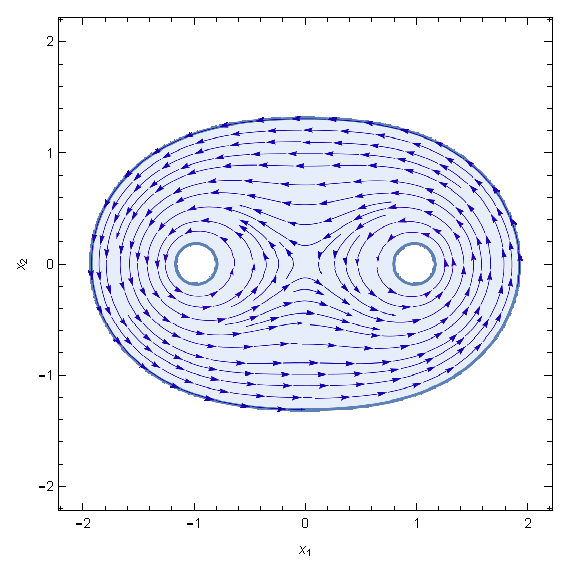
\includegraphics[width=0.7\textwidth]{../Plots/HarmonicVectorFields_gr1.eps}
  \caption{A plot of $u=\nabla^\perp\psi$ in the region $\psi^{-1}\brk*{[-1,1]}$.
    Here $\psi$ is given by equation \eqref{eq:n2:hvf:noInflowNoOutflow}.}
  \label{pl:n2_hvf_noInflowNoOutflow}
\end{figure}

In a second example given by \cite{Wahlen2023} we fix the domain rather than the function.
For this set $\overline{\Omega}=\overline{B_4}\setminus\brk*{B_1(2e_1)\cup B_1(-2e_1)}$ to be the domain.
We then have the system
\begin{equation}
  \begin{aligned}
    \Delta \psi&=0 &&\text{, on }\Omega \\
    \psi&=0 &&\text{, on the outer ring }4S^1 \\
    \psi&=1 &&\text{, on the inner rings }S^1(-2e_1)\cup S^1(2e_1)
  \end{aligned}\label{eq:n2:hvf:roundRegion:noInflowNoOutflow}
\end{equation}
We solve this system numerically and set $u=\nabla^\perp\psi$.
The result is plotted in figure \ref{pl:n2_hvf_roundRegion_noInflowNoOutflow}.
\begin{figure}
  \centering
  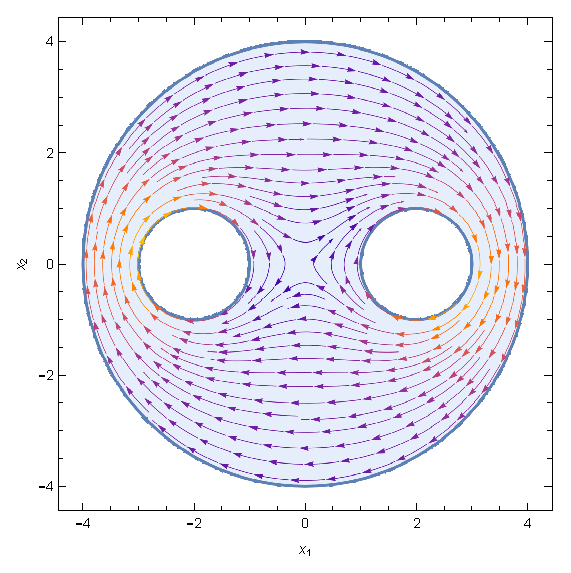
\includegraphics[width=0.7\textwidth]{../Plots/HarmonicVectorFields_gr4.eps}
  \caption{A plot of $u=\nabla^\perp\psi$ where $\psi$ is the numerical solution to
   \eqref{eq:n2:hvf:roundRegion:noInflowNoOutflow}.}
  \label{pl:n2_hvf_roundRegion_noInflowNoOutflow}
\end{figure}

\subsection{An example of inflow on one side and outflow on the other}
In the following we aim to give examples of domains in $d=2$ dimensions for which 
we have inflow on one simply connected boundary component and outflow on another simply connected boundary
component.
For this consider first the stream function
\begin{equation}
  \begin{aligned}
  \psi\colon \R^2\setminus\brk[c]*{-e_1,e_1}&\to\R^2 \\
  x&\mapsto\Phi_2\brk*{x-e_1}+x_1
  \end{aligned}\label{eq:n2:hvf:InflowOutflow:singleHole}
\end{equation}
Figure \ref{pl:n2_hvf_InflowOutflow_asymmetric_single} indicates that $u=\nabla^\perp\psi$ fulfills the
requirements.
\begin{figure}
  \centering
  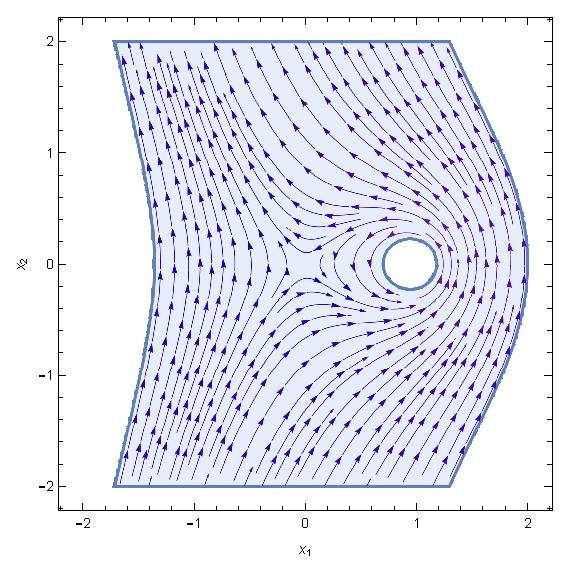
\includegraphics[width=0.7\textwidth]{../Plots/HarmonicVectorFields_gr3.eps}
  \caption{A plot of $u=\nabla^\perp\psi$ in the region $\psi^{-1}\brk*{[-0.5,2]}\cap \R\times[-2,2]$.
  Here $\psi$ is given by equation \eqref{eq:n2:hvf:InflowOutflow:singleHole}.}
  \label{pl:n2_hvf_InflowOutflow_asymmetric_single}
\end{figure}

Now we would like to have a harmonic vector field similar to the example with two holes with
inflow on the one side and outflow on the other. 
For this consider the streamline
\begin{equation}
  \begin{aligned}
  u\colon\R^2\setminus\brk[c]*{-e_1,e_1}&\to\R^2 \\
  x&\mapsto\Phi_2\brk*{x-e_1}-\Phi_2\brk*{x+e_1}+x_1
  \end{aligned}\label{eq:n2:hvf:noInflowNoOutflow:doubleHoles}
\end{equation}
Figure \ref{pl:n2_hvf_InflowOutflow_symmetric_region} indicates that $u=\nabla^\perp\psi$ is the function
we are looking for.
\begin{figure}
  \centering
  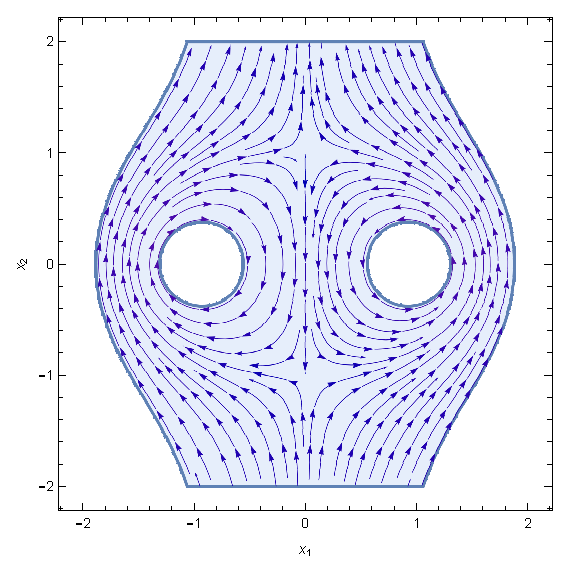
\includegraphics[width=0.7\textwidth]{../Plots/HarmonicVectorFields_gr2.eps}
  \caption{A plot of $u=\nabla^\perp\psi$ in the region $\psi^{-1}\brk*{[-0.7,0.7]}\cap \R\times[-2,2]$.
  Here $\psi$ is given by equation \eqref{eq:n2:hvf:noInflowNoOutflow:doubleHoles}.}
  \label{pl:n2_hvf_InflowOutflow_symmetric_region}
\end{figure}


In another example given by \cite{Wahlen2023} we once again fix the domain rather than the function.
Let $\Omega=B_4\setminus\brk*{B_1(2e_1)\cup B_1(-2e_1)}$ be the domain as before.
We now have the system
\begin{equation}
  \begin{aligned}
    \Delta \psi&=0 &&\text{, on }\Omega \\
    \psi&=0 &&\text{, on the outer ring }4S^1 \\
    \psi&=-1 &&\text{, on the left inner ring }S^1(-2e_1) \\
    \psi&=1 &&\text{, on the right inner ring }S^1(2e_1)
  \end{aligned}\label{eq:n2:hvf:roundRegion:InflowOutflow}
\end{equation}
We solve this system numerically and set $u=\nabla^\perp\psi$.
The result is plotted in figure \ref{pl:n2_hvf_roundRegion_InflowOutflow}.
\begin{figure}
  \centering
  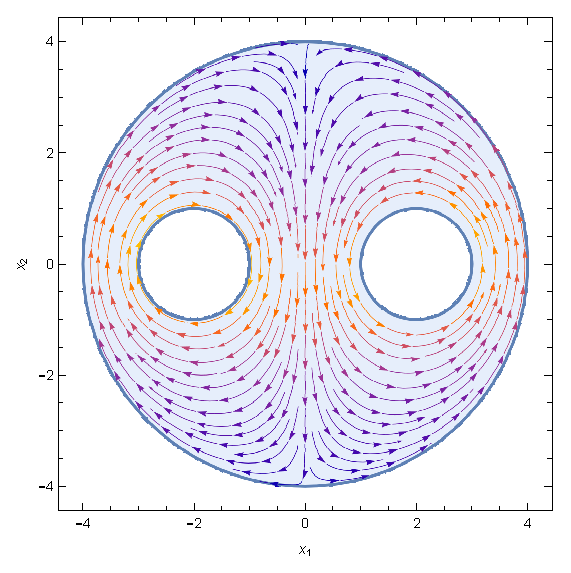
\includegraphics[width=0.7\textwidth]{../Plots/HarmonicVectorFields_gr5.eps}
  \caption{A plot of $u=\nabla^\perp\psi$ where $\psi$ is the numerical solution to
   \eqref{eq:n2:hvf:roundRegion:InflowOutflow}.}
  \label{pl:n2_hvf_roundRegion_InflowOutflow}
\end{figure}
\td{Check the signs of this example. Give explanation for why it works.}

\newpage

\section{Harmonic functions, $d=3$}

\subsection{The cylinder}

The following proof comes from \cite{Wahlen2023}
\begin{proposition}
  Let $\Omega=(0,1)\times B_1\subseteq\R^3$ be the cylinder. Let further $f\colon\overline{\Omega}\to\R$ be regular 
  harmonic with no inflow or outflow on the sides 
  $\partial (0,1)\times B_1$, no outflow on $\brk[c]{0}\times B_1$ and no inflow on $\brk[c]{1}\times B_1$. 
  Then $f$ cannot have a critical point.
\end{proposition}
\begin{proof}
  Assume not. Since
  \begin{align*}
    \Delta(\partial_1f)=\partial_1(\Delta f)=0
  \end{align*}
  we have by the maximum principle that $\partial_1 f$ attains its minimum on the boundary $\Sigma$. Since $\partial_1 f(x)=0$ for some interiour point 
  by assumption and $\partial_1 f>0$ on the lids $\brk[c]{x_1=0}\cup\brk[c]{x_1=1}$ there exists a point
  $x\in(0,1)\times S^1$ such that $\partial_1f(x)$ is minimal on $\overline{\Omega}$. But then we have by Hopf's lemma
  that
  \begin{align*}
    0<\nabla (\partial_1f)\cdot n=\partial_1(\nabla f\cdot n)=0\,,
  \end{align*}
  a contradiction.
\end{proof}

\newpage

\subsection{Harmonic vector fields, $d=3$}
We obtain as a quick consequence of the hairy ball theorem
\begin{proposition}
  Let $\Omega$ have Betti numbers $R_0$, $R_1$ and $R_2$.
  Let $u\colon\overline{\Omega}\to\R$
  be a regular harmonic vector field without inflow or outflow. Then we have
  \begin{align*}
    R_2\leq R_1\,.
  \end{align*}
\end{proposition}
\begin{proof}
  Assume not. Since $\Omega$ has $R_2$ bubbles and $R_1$ holes there exists by the pidgeon hole
  principle a bubble $\Gamma\subseteq\Sigma$ without a hole. Since $u$ has no inflow or outflow on $\Gamma$ we
  have that the restriction $u\vert_\Gamma\in T\Gamma$ is a vector field on $\Gamma$. Since $u$ is regular
  $u\vert_\Gamma$ does not vanish. But $\Gamma$ is homeomorphic to the Ball in contradiction to the hairy ball theorem.
\end{proof}\ruggedtodo[]{A little more rigour would not harm.}
Mimicking the proof in 2 dimensions we obtain the following proposition.
\begin{proposition}
  Let $\Omega$ have Betti numbers $R_0$, $R_1$ and $R_2$.
  Let $u\colon\overline{\Omega}\to\R$ be a regular harmonic vector field without inflow or outflow. Then we have the following relation for
  critical points of $u$
  \begin{align*}
    M_2=M_1
  \end{align*}
\end{proposition}
\begin{proof}[Attempt at proof.]
  As in the two-dimensional case we begin by cutting up the domain such that the slit domain is homeomorphic to the ball with bubbles.
  Once again by proposition \ref{pr:n2:hvf:simplyConnected} $u$ is the gradient of a harmonic function $u$ on this new domain.
  $f$ has no critical points on the boundary $\Sigma$ and on the cut boundary it fulfils the conditions
  \begin{align}
    \mu_0=\nu_2\qquad \mu_1=\nu_1 \qquad \mu_2=\nu_0 \label{eq:n3:hvf:relationsMuNu}
  \end{align}
  by the same reasoning. We now have the Morse inequalities for $f$ and $-f$
  \begin{align}
    M_2+\mu_2-R_2-M_1-\mu_1+R_1+\mu_0-R_0=0 \label{eq:n3:hvf:MorseInequalities:1} \\
    M_1+\nu_2-R_2-M_2-\nu_1+R_1+\nu_0-R_0=0 \label{eq:n3:hvf:MorseInequalities:2}
  \end{align}
  It then follows by subtracting equation \eqref{eq:n3:hvf:MorseInequalities:2} from \eqref{eq:n3:hvf:MorseInequalities:1}
  and using relations \eqref{eq:n3:hvf:relationsMuNu} that
  \begin{align*}
    2\brk*{M_2-M_1}=0\,.
  \end{align*}
\end{proof}\ruggedtodo[]{Introduce Morse inequalities for $-f$.}


\newpage

\subsection{Harmonic functions, $d=4$} 
Define the harmonic function 
\begin{align*}
  f\colon B_1\subseteq\R^4&\to \R \\
  x &\mapsto x_1^2+x_2^2-x_3^2-x_4^2\,.
\end{align*}
This has a stagnation point at the origin. We now claim that the sets $\Sigma^+$ and $\Sigma^-$ are both simply connected, i.e.\
we have a tube in $\R^4$ with throughflow and a stagnation point.

\begin{proof}
To prove this claim we observe that the boundary $\partial B_1$ can be parametrised by the coordinates $\bx = (x_2,x_3,x_4)$
for which we have $\abs{\bx}\leq 1$. By the condition
\begin{align}
  \sum_i x_i^2 = 1\label{eq:n4:ball}
\end{align}
on the boundary $\partial B_1$ we have that $x_1$ is then uniquely determined up to sign. Thus we have have defined parametrisations
\begin{align}
  \begin{aligned}\phi_\pm\colon B_1\subseteq\R^3&\to\R \\
  \bx&\mapsto x\text{ such that } \pm x_1\geq0
  \end{aligned}\label{eq:n4:parametrisation}
\end{align}
with inverses $\psi_\pm = \brk*{\phi_\pm}^{-1}$.
We now calculate the gradient of $f$
\begin{align*}
  \nabla f = 2\vect{x_1 & x_2 & -x_3 & -x_4}^\top
\end{align*}
and the normal to $\partial B_1$
\begin{align*}
  n = \vect{x_1 & \cdots & x_4}^\top\,.
\end{align*}
Thus we have $x\in\Sigma^\pm$ iff
\begin{align*}
  0<\pm \nabla f\cdot n = \pm 2\brk*{x_1^2+x_2^2-x_3^2-x_4^2}
\end{align*}
Using condition \eqref{eq:n4:ball} we obtain the equivalent condition
\begin{align*}
  0<\pm 1-2\brk*{x_3^2+x_4^2}
\end{align*}
Define the cylinder
\begin{align*}
  C = \brk[c]*{\bx\in \R^3\colon x_3^2+x_4^2<1/2} = \R\times B_{1/\sqrt{2}}
\end{align*}
If we return to our parametrisation \eqref{eq:n4:parametrisation} we see that we have $\bx\in B_1\cap C$ iff
$\phi_\pm(x)\in \Sigma^+$ and hence 
\begin{align*}
  B_1\cap C=\psi_\pm\brk*{\Sigma^+}\,.
\end{align*}
Analogously  we have 
\begin{align*}
  B_1\setminus C=\psi_\pm\brk*{\Sigma^-}\,.
\end{align*}
The claim then follows from the fact that $\phi$ is a homeomorphism onto its image and $x_1=0$ is 
equivalent to $\bx\in \partial B_1\subseteq \R^2$. The situation is depicted in figure \ref{fi:n4_sigma}.

\td{Check that the transition at the boundary is legal.}
\begin{figure}[h]
  \centering
  \def\svgwidth{0.7\textwidth}
  \input{../Figures/n4_sigma.pdf_tex}
  \caption{Visualisation of the situation.}
  \label{fi:n4_sigma}
\end{figure}
\end{proof}

\clearpage

% \printnomenclature


\glsaddall
\printunsrtglossary[type=symbols,style=long]

\clearpage

% TODO: potentially add Irwin, smooth dynamical systems
% \section{Bibliography}
\nocite{*}
%Main source
%\printbibliography[heading=none, keyword={main}]
%\noindent Other sources
\printbibliography


\end{document}